\documentclass[a4paper,11pt]{article}
\usepackage{fullpage}

\usepackage{amsmath}
\usepackage{amsfonts}
\usepackage{amssymb}
\usepackage{amsthm}
\usepackage{mathtools}

\usepackage{graphicx}

\newcommand{\assignmentname}{COMP2911 Assignment 2}
\newcommand{\coursename}{COMP2911}

\usepackage{fancyhdr}
\pagestyle{fancy}
\setlength{\headheight}{15.2pt}
\setlength{\headsep}{16pt}
\fancyhf{}
\fancyhead[L]{\textsc{Evgeny Martynov}}
\fancyhead[C]{\coursename}
\fancyhead[R]{\texttt{z3301707}}
\fancyfoot[L]{\textsc{\assignmentname}}
\fancyfoot[R]{\thepage}

\begin{document}

\section*{Class diagram}

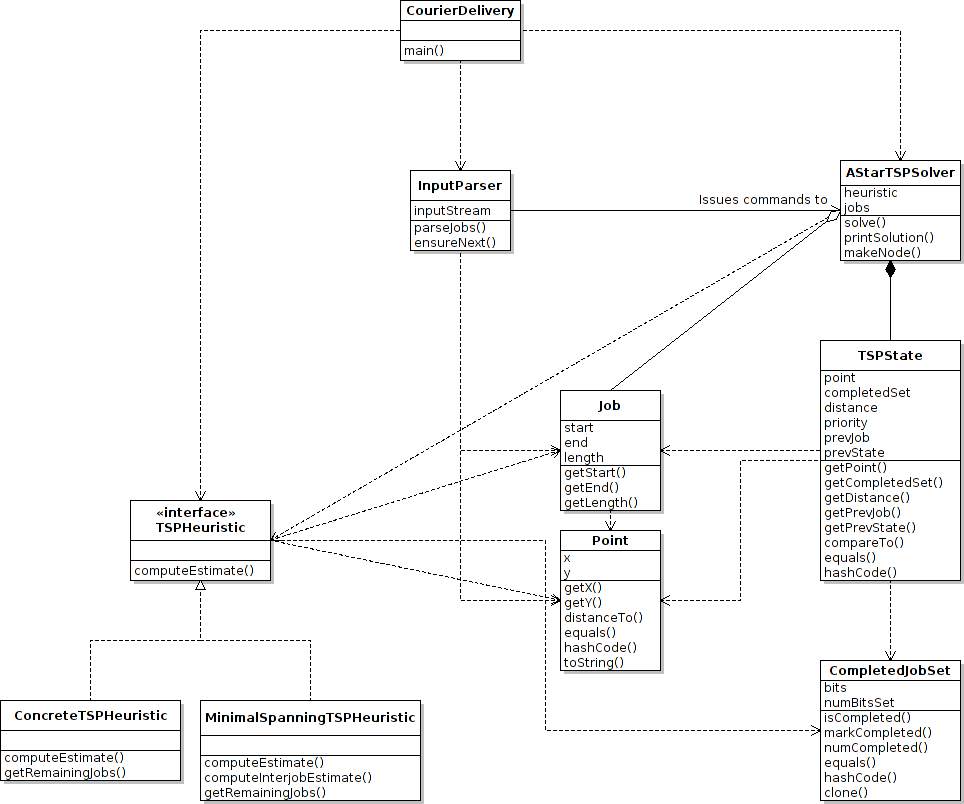
\includegraphics[scale=0.5]{uml.png}
\vspace{5mm}

Note that in the above diagram, we do not include method names for constructors
(they are implied and present in all classes).

Further, dependencies are drawn between the \texttt{TSPHeuristic} interface and
the rest of the classes, and not between \texttt{ConcreteTSPHeuristic} and the
rest of the classes. The dependencies are the same as for its interface.

Classes \texttt{Job} and/or \texttt{Point} are semi-utility classes, and hence
everything seems to rely on them. If we were to draw a real UML diagram and not
the one COMP2911 expects, we probably would not show these classes on this page.

Further, note the Strategy pattern in use for the \texttt{TSPHeuristic}. It may
not be apparent due to only having a single concrete class for the interface,
but it does conform to the pattern.

\end{document}
